\section{Auswertung}
\label{sec:Auswertung}

Im Folgenden wir der Mittelwert allgmein über die Formel \begin{equation}
    \mu = \frac{1}N \sum_{n=1}^N x_n
    \label{eqn:mw}   
\end{equation} berechnet. Für die Standardabweichung gilt \begin{equation}
    \sigma = \sqrt{\frac{1}{N-1} \sum_{n=1}^N (x_n -\mu)^2}
    \label{eqn:std}
\end{equation}

\subsection{Winkelrichtgröße}
Als erstes wird die Winkelrichtgröße der Torsionsfeder berechnet.
Durch passendes Umstellen und Einsetzen der Gleichungen \eqref{eqn:T} und \eqref{eqn:M} ergibt sich die Gleichung
\begin{equation*}
    D=\frac{Fr}{\phi}.
    \end{equation*}
Mit Hilfe der Daten der Tabelle \:\ref{tab:1} errechnet sich die Winkelrichtgröße zu $D=\SI{0.022(001)}{\newton\m}$.
\begin{table}
    \centering 
    \caption{Daten zur Bestimmung der Winkelrichtgröße.}
    \label{tab:1}
    \begin{tabular}{S S}
        \toprule
        {$\phi$ in Grad} & {$F \:/\: \si{\newton}$} \\
        \midrule
        20 & 0.060 \\
        30 & 0.100 \\
        40 & 0.155 \\
        50 & 0.195 \\
        60 & 0.260 \\
        70 & 0.300 \\
        80 & 0.350 \\
        90 & 0.380 \\
        
        \bottomrule
    \end{tabular}
\end{table}

\subsection{Eigenträgheitsmoment}

\begin{table}
    \centering 
    \caption{Daten zur Bestimmung des Eigenträgheitsmomentes.}
    \label{tab:2}
    \begin{tabular}{S S}
        \toprule
        $r \:/\: \si{\centi\meter}$ & $T \:/\: \si{\s}$ \\
        \midrule
        2.5 & 2.34  \\
        4.0 & 2.52    \\
        6.0 & 2.83    \\
        8.0 & 3.20    \\
        10.0 & 3.50   \\
        12.0 & 4.00   \\
        14.0 & 4.50   \\
        16.0 & 5.05   \\
        18.0 & 5.55   \\
        20.0 & 6.10   \\
        22.0 & 6.60   \\
        
        \bottomrule
    \end{tabular}
\end{table}


Das Eigenträgheitsmoment $I_D$ des Aufbaus lässt sich aus dem Gesamtträgheitsmoment 

    \begin{equation}
    I_{\text{ges}}=2\cdot m r^2 +I_D
    \label{eqn:Iges}
    \end{equation}

bestimmen. Dazu wird eine lineare Regression auf $T^2$ und $r^2$ aus der Tabelle \:\ref{tab:2} verwendet:

    \begin{equation*}
        T^2=a\cdot r^2+b
    \end{equation*}
Durch Einsetzen der Gleichung \eqref{eqn:Iges} in die quadrierte Form der Gleichung \eqref{eqn:T} folgt die Gleichung
    \begin{equation*}
        T^2=4\pi^2\frac{I}{D}=\frac{(2mr^2+I_D)4\pi^2}{D}=\frac{8m\pi^2}{D}r^2+\underbrace{\frac{4\pi^2I_D}{D}}_{= b}.
    \end{equation*}
Der Teil $b$ enthält das zu bestimmende Eigenträgheitsmoment. Die Ausgleichsgerade aus der Abbildung \:\ref{fig:gerade}
liefert den Parameter $b$, womit sich schließlich über
    \begin{equation}
        I_D=\frac{bD}{4\pi^2}
        \label{eqn:eig}
    \end{equation}
das Eigenträgheitsmoment des Aufbaus bestimmen lässt. Mit dem Geradenparametern $a=\num{801(6)}$ und $b=\num{4.85(15)}$ ergibt sich das Eigenträgheitsmoment \begin{equation}
    I_D=\num{276(015)e-5}\,\si{\kilo\gram\square\m}.
\end{equation}

\begin{figure}
    \caption{Messwerte zum bestimmen des Eigenträgheitsmomentes.}
    \centering
    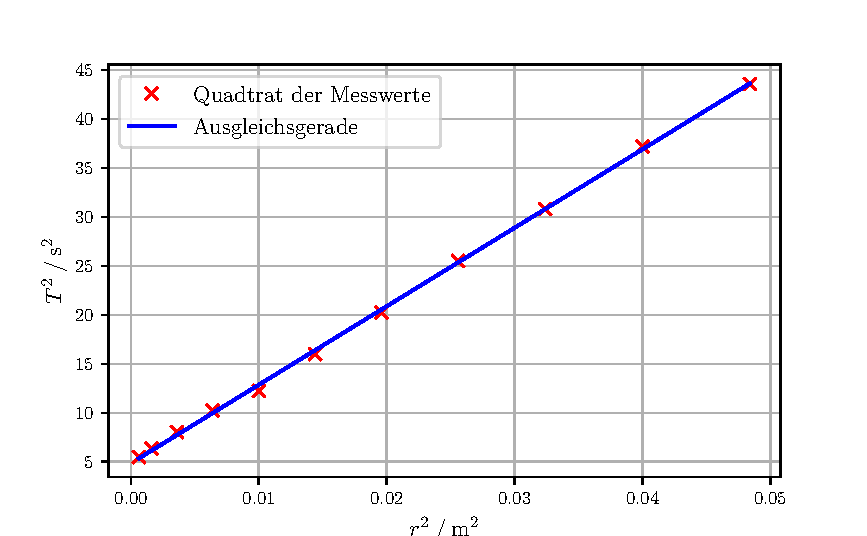
\includegraphics[height=8cm]{build/Ausgleichsgerade.pdf}
    \label{fig:gerade}
\end{figure}


\subsection{Trägheitsmoment der Zylinder}

Die Periodendauer der Schwingung der beiden Zylinder werden in der Tabelle\:\ref{tab:t_zyl} gezeigt. 
$T_\text{sym}$ gilt für die Drehung um die 
Symmetrieachse und $T_\text{asym}$ gilt für die andere Achse, wie sie auch in Bild\:\ref{fig:Probekoerper} zu sehen ist.

\begin{table}
    \centering
    \caption{Periodendauer der Zylinder}
    \label{tab:t_zyl}
    \begin{tabular}{S S}
        \toprule
        $T_\text{sym}\:/\:\si{\s}$ & $T_\text{asym}\:/\:\si{\s}$ \\
        \midrule
        1.22 & 0.91 \\
        1.26 & 0.89 \\
        1.30 & 0.89 \\
        1.21 & 0.92 \\
        1.24 & 0.93 \\
        \bottomrule
    \end{tabular}
\end{table}

Über die Gleichung\:\ref{eqn:mw} kann der Mittelwert für die jeweiligen $T$ bestimmt werden:
\begin{align}
    T_\text{sym}& = 1.246\pm 0.016 \si{\s} \\
    T_\text{asym}&= 0.908\pm 0.008 \si{\s}
\end{align}

Damit lässt sich für beide Zylinder, unter Beachtung des durch Gleichung\:\ref{eqn:eig} berechnete Eigenträgheitsmoments, jeweils deren
Trägheitsmomente berechnen. Die jeweiligen $I$ sind analog zu ihren Periodendauern gekennzeichnet. Die experimentell bestimmten
Trägheitsmomente ergeben sich somit zu: 
\begin{align}
I_\text{sym}& = \num{-1,88(16)e-3}\,\si{\kilo\gram\square\m} \\
I_\text{asym}& = \num{-2,29(15)e-3}\,\si{\kilo\gram\square\m}
\end{align}

Die Theoriewerte lassen sich mit den Gleichungen aus der Abb\:\ref{fig:probe} berechnen:

\begin{align}
I_\text{sym,th}& = \num{0.786e-3}\,\si{\kilo\gram\square\m} \\
I_\text{asym,th}& = \num{0.477e-3}\,\si{\kilo\gram\square\m}
\end{align}

\subsection{Trägheitsmomente der Puppe}
\begin{table}
    \centering 
    \caption{Periodendauer bei beiden Puppenpositionen.}
    \label{tab:3}
    \begin{tabular}{S S}
        \toprule
        \multicolumn{2}{c}{T \:/\: \si{\s}}\\
        \cmidrule(lr){1-2}
        {Pos. 1} & {Pos. 2} \\
        \midrule
        0.61 & 0.95 \\
        0.63 & 0.96 \\
        0.66 & 0.96 \\
        0.65 & 0.93 \\
        0.66 & 0.97 \\
        \bottomrule
    \end{tabular}
\end{table}

Aus den Werten der Tabelle \:\ref{tab:3} lassen sich die gemittelten Periodendauern der einzelnen Puppenpositionen bestimmen. Diese ergeben sich bei Position 1 zu $T_{\text{p1}}=\SI{0.642(010)}{\s}$ und bei Position 2 zu $T_{\text{p2}}=\SI{0.954(007)}{\s}$. Durch Umstellen der Gleichung \eqref{eqn:T} und unter Beachtung des Eigenträgheitsmomentes des Aufbaus kommt es zu der Gleichung
\begin{equation}
    I=\frac{DT^2}{4\pi^2}-I_D,
\end{equation}
mit welcher die Trägheitsmomente der verschiedenen Positionen in Abhängigkeit der jeweiligen Periodendauer errechnet werden können.
Diese ergeben sich damit zu \begin{equation}
    I_{\text{exp,Pos1}}=\num{-2,52(14)e-3}\,\si{\kilo\gram\square\m}
\end{equation} und \begin{equation}
    I_{\text{exp,Pos2}}=\num{-2,24(13)e-3}\,\si{\kilo\gram\square\m}.
\end{equation}


\begin{table}
    \centering 
    \caption{Maße der Zylinder zur Näherung des Puppenvolumens.}
    \label{tab:4}
    \begin{tabular}{S S S}
        \toprule
        & {Durchmesser $d\:/\: \si{\centi\m}$} & {Höhe $h\:/\: \si{\centi\m}$} \\
        \midrule
        \text{Kopf} & 2.1 & 5.0 \\
        \text{Rumpf} & 3.8 & 9.5 \\
        \text{Bein} & 1.5 & 15.0 \\
        \text{Arm }& 1.3 & 13.5 \\
        \bottomrule
    \end{tabular}
\end{table}


\begin{table}
    \centering 
    \caption{Volumina der Zylinder zur Näherung des Puppenvolumens.}
    \label{tab:5}
    \begin{tabular}{S S}
        \toprule
        & {Voulmen $V\:/\: \si{\cubic\centi\m}$} \\
        \midrule
        \text{Kopf} & 17.318 \\
        \text{Rumpf} & 107.741 \\
        \text{Bein} & 26.507 \\
        \text{Arm} & 17.919 \\
        \text{Insgesamt} & 213.911 \\
        \bottomrule
    \end{tabular}
\end{table}

Da die Puppe näherungsweise aus einer Zusammenstellung verschiedener Zylinder besteht wird das Volumen der Puppe ebenfalls durch die Summe einzelner Zylindervolumina zusammengesetzt. Die jeweiligen Maße können der Tabelle \:\ref{tab:4} entnommen werden. Aus diesen Maßen lassen sich die Volimina der einzelnen Zylinder über die Gleichung \eqref{eqn:Z} berechnen. Die Ergebnisse sind in Tabelle \:\ref{tab:5} aufgeführt.
Das Gesamtvolumen der Puppe ist somit $V_{\text{ges}}=\SI{213.911}{\cubic\centi\m}$. 
Da das Verhältis zwischen Gesamtmasse, Gesamtvolumen und Teilvolumen der einzelnen Körperteile der Puppe bekannt sind, lässt sich über die Gleichung
\begin{equation*}
    m_{\text{körperteil}}=\frac{V_{\text{körperteil}}}{V_{\text{ges}}}m_{\text{ges}}
\end{equation*}
das Gewicht jedes einzelnen Körperteiles bestimmen. 


\begin{table}
    \centering 
    \caption{Theoretische Trägheitsmomente der Puppe in beiden Positionen.}
    \label{tab:6}
    \begin{tabular}{S S S}
        \toprule
        & \multicolumn{2}{c}{Trägheitsmoment $I_{\text{th}}\:/\: \si{\kilo\gram\square\m}$} \\
        \cmidrule(lr){1-3}
        & {Pos. 1} & {Pos. 2} \\
        \midrule
        \text{Kopf}  &\num{0.0750e-5} & \num{0.0750e-5}\\
        \text{Rumpf} &\num{1.5273e-5} & \num{1.5273e-5}\\
        \text{Beine} &\num{0.6774e-5} & \num{31.836e-5}\\
        \text{Arme}  &\num{25.364e-5} & \num{25.364e-5}\\
        \text{Insgesamt} &\num{27.6339714e-5} &\num{58.8024788e-5}\\
        \bottomrule
    \end{tabular}
\end{table}


Die theoretischen Trägheitsmomente der beiden Puppenpositionen können nun, mit der Kenntnis über die einzelnen Massen der Körperteile, über die Formeln aus Abbildung \:\ref{fig:probe} bestimmt werden. 
Da sowohl die Rotationsache der Arme als auch Beine der Puppe nicht durch den jeweiligen Schwerpunkt führt, wird der Satz von Steiner
\eqref{eqn:stein} zum Berechnen der Trägheitsmomente verwendet. Das Gesamtträgheitsmoment der Puppe ergibt sich dann über die Summe aller Einzelträgheitsmomente, welche in Tabelle \:\ref{tab:6} aufgeführt sind.
So ergibt sich ein Trägheitsmoment \begin{equation}
    I_{\text{th,Pos.1}}=\num{27.63e-5}\,\si{\kilo\gram\square\m}
\end{equation} für Position 1 und ein Trägheitsmoment \begin{equation}
    I_{\text{th,Pos.2}}=\num{58.80e-5}\,\si{\kilo\gram\square\m}
\end{equation}
für Position 2.
%Messwerte: Alle gemessenen physikalischen Größen sind übersichtlich darzustellen.
%
%Auswertung:
%Berechnung der geforderten Endergebnisse
%mit allen Zwischenrechnungen und Fehlerformeln, sodass die Rechnung nachvollziehbar ist.
%Eine kurze Erläuterung der Rechnungen (z.B. verwendete Programme)
%Graphische Darstellung der Ergebnisse
